\documentclass[12pt]{article}
\usepackage{verbatim}
\usepackage[dvips]{epsfig}
\usepackage{color}
\usepackage{url}
\usepackage[colorlinks=true]{hyperref}

\begin{document}

\section*{GENESIS: Documentation}

{\bf Related Documentation:}
% start: userdocs-tag-replace-items related-cbi-architecture
% end: userdocs-tag-replace-items related-cbi-architecture

\section*{The CBI Simulator Framework in a Multi-Scale Modeling Context}

\subsection*{structure}

- problem statement: multi-scale modeling requires a single model-container

- explain CBI architecture

- apply: G-3 and scripting

- explain communication infrastructure for multi-scale modeling


\subsection*{Multi-Scale Modeling and the User-Workflow}
The user-workflow is a simple workflow based on experimental paradigm
to allow experimentalists access to neuronal simulation.  In contrast,
the number of available numerical algorithms is large.  As a
consequence any tool will become useful as far as its implicit or
explicit capacity of simplifying the mapping from this large set of
techniques to the simple user-workflow.  Currently such a tool does
not exist.  This is at the core of the problem of multi-scale
simulation.

A major benefit of the CBI framework is that its decomposes into
self-contained modules that have a simple correspondence with the
user-workflow.

It succeeds in simplifying a substantial part of the picture: running
either a simulation of a single neuron or of a network of
multicompartmental neurons can be done from the command line (and uses
many implicit default values).  Advanced G-3 users can drill down into
the details of and make changes to either the model, the experiment or
the simulation configuration.  How to expand the G-3 scope for
multi-scale simulation is explained below.

It is simple to run simulations from a command line.  As an example:

ssp --cell cells/purkinje/edsjb1994.ndf --inject-current 1e-9 --time 1

ssp --network networks/spiker3.ndf --network-input 1e-9 --time 1

Both these command lines follow a template of model specification,
experiment specification, simulation configuration.  Note that line 2
is essentially a simple multi-scale simulation that instantiates
solvers and run-time data communication components as necessary.  By
design this feature of the modular architecture of NS / G-3 works the
same within and across all scales.

The question 'given all the technology available, why is multi-scale
modeling so difficult?' is quickly and superficially answered after
the observation that simulations are limited by their engines and
solvers.

A good use case is necessary to make this understandable, ie the three
steps in your email.

$<$based on such as use case it is easy to make a diagram for further
clarification during a presentation about these three steps, and it
can have three 'growing' versions during the presentation where each
version of the diagram plugs in new software components into the
system$>$

I think a presentation should have the following implicit elements:

1. the user-workflow: a scientist first cares about the scientific
question, the technology is secondary.

2. the model and its computational expression have a central role from
the science viewpoint (so the requirement for having exactly one
model-container).  At its essence a scientific model is 'scale-less'
(but some people will not like this type of expression), or worded
differently, the expression of the model can be independent of scale,
and so can be multi-scale, or not (but a scientist does not care
because he simply implements the simple user-workflow during his daily
work).

3. the single model-container 'contains' the model with both
structures of components and values.  It has all the connections
between the different components of the model, independent of whether
these components are solved independently / in isolation or,
alternatively, by a single engine.

The G-3 plugin mechanism interfaces the (single) model-container with
multiple run-time simulation objects.  Superficially there is a
discrete event system (action potential propagation abstraction and
communication), a compartmental solver (crank-nicolson or simpler),
and may be a kinetic pathway solver (RK or equivalent).  This is what
G-2 offers (but without a rigid user-workflow).  When you go one level
down, we encounter a rich set of well understood equations that can be
solved deterministically or stochastically (Monte-Carlo or otherwise).
 This landscape is more complex, although mathematically relatively
well understood.

Some of the equation types in subcellular simulations:
- K-Epsilon
- Navier-Stokes
- Heat-equations
- Reynold-equations
- Helmholtz-equations
- Poisson-Boltzmann equations
(note that not all these names apply to neuroscience I can update the
list for neuroscience):

Looking one level up, we see an equally rich set of gamble-and-win
solution methods:

Some of the model-types in supranetwork (large scale) simulations:
- IaF
- Adaptive IaF
- Izhekevic IaF
- Conductance based synapses
- Current based synapses
- Convolution and Waveform dependent synaptic weights

Two conclusions can be drawn: firstly from the biology point of view
the single neuron level seems to be the level that is best understood,
the anchor point for further expansion.  Firstly, in comparison to
most of the other software tools, this puts G-3 in an excellent
strategical position.  Both the Neuron and Moose simulators seem to be
in slightly different but mostly equivalent positions.

Secondly it is clear that the old generation of simulators (not
including G-3) does not offer the flexibility required to suit the
next generation of multi-scale models because of the complexity of the
available solution methods.  In other words current software
technology limits the scope of the research.  Many people agree with
the statement, but few truly understand and even fewer are trying to
change that situation, so I think it is important to make that point
clear.

$<$technical intermezzo$>$

Besides our efforts there are two other efforts that I am aware of
that try to solve this problem.  Firstly Neuron now includes
additional solvers for subcellular modeling.  I have strong personal
doubts that this will be truly successful for two reasons: the Neuron
environment does not have a mature plugin mechanism (read: it is
previous generation).  As a consequence the new solvers are tightly
integrated with the rest of the code and new solvers cannot be
contributed by external developers.  It also seems that the networking
capabilities in Neuron are still immature from a usability
perspective.  Overall I have the impression that Neuron is at the
limits of its internal (monolythic) architecture.

Secondly Moose also has a plugin architecture that allows developers
to plugin new solvers but it is immature.  The API is unstable
(changes over time) and is hardly documented.  The API is based on the
mathematics of the model (via the Moose messaging system) which is
conceptually similar to G-2 and I consider it a limiting factor.

In part because of these problems with Moose and Neuron for
multi-scale simulation, it is clear now that advanced middle-ware is /
will be necessary for the implementation of efficient communication
between solvers.  Currently people try to hack in the middle-ware as
necessary, but neither Neuron nor Moose nor any other simulator I
know, offers the handles necessary to manage this type of middle-ware
at run-time.  G-3 does and it works.  As a proof of concept, Mando
recently started to interface with these handles without understanding
their full scope (because he does not have to).  But except for the
model-container there are no G-3 components nor middle-ware available
for running multi-scale simulations.  So it currently stays a proof of
concept.

$<$end technical intermezzo$>$

For a presentation:

1. Contrast the complexity of a Purkinje cell (early in the
presentation) with that of the user-workflow-to-simulation mapping
(later in the presentation, eg. a slide that lists some of the
available solution methods, I do have such a slide somewhere in one of
my own presentations, let me know whether you would like to see / use
it).

2. The complexity we are facing is similar to multi-scale simulation
in other fields.  Nevertheless the pressure of the complexity of
biology by itself has a multiplicative factor to the already present
mathematical complexity.

Some additional interesting points:

1. The degree of how much a G-3 user drills down into technical
details of a simulation puts in him in one of the categories of either
student, teacher or researcher role, essentially on a mapping ranging
from the most naive to the most advanced role.  G-3 makes this
distinction rather intuitive.  The documentation system expands on
this idea.

2. Complementary to the scales starting from molecules upto system
networks, and I think as interesting, is the comparative study.

Let me know if I can be of further help.  Specifically if you want me
to send you some slides.

\vspace{1cm}

{\LARGE Start of paper here ----------}

\section*{Introduction}

Three possible definitions of multi-scale modeling.

There are two common definitions

1. biologically inspired definition (eg. model involves a network and
detailed channel models).

2. mathematically inspired definition (eg. use cable equations,
discrete event models for axonal propagation, and HH equations for the
channels).

Both definitions may mean that 99\% of the models out there is already
multi-scale, rendering those definitions void of meaning.

{\LARGE include here one of the multi-scale figures here (NS based,
  Jim's, or other?).  It will make the point that many more
  definitions are possible.}

new definition, definition used in this paper, based on software
principles and separation of concerns (CBI-architecture):

3. software definition: based on the CBI architecture: the application
of a model for simulation or otherwise, that is contained by a single
software entity (a single model-container), but using solvers that
implement different mathematical tools and that communicate with one
another during run-time using the communication infrastructure
provided by the CBI architecture
(figure~\ref{fig:mental-model-simulation-path}).


\begin{figure}[ht]
  \begin{center}
    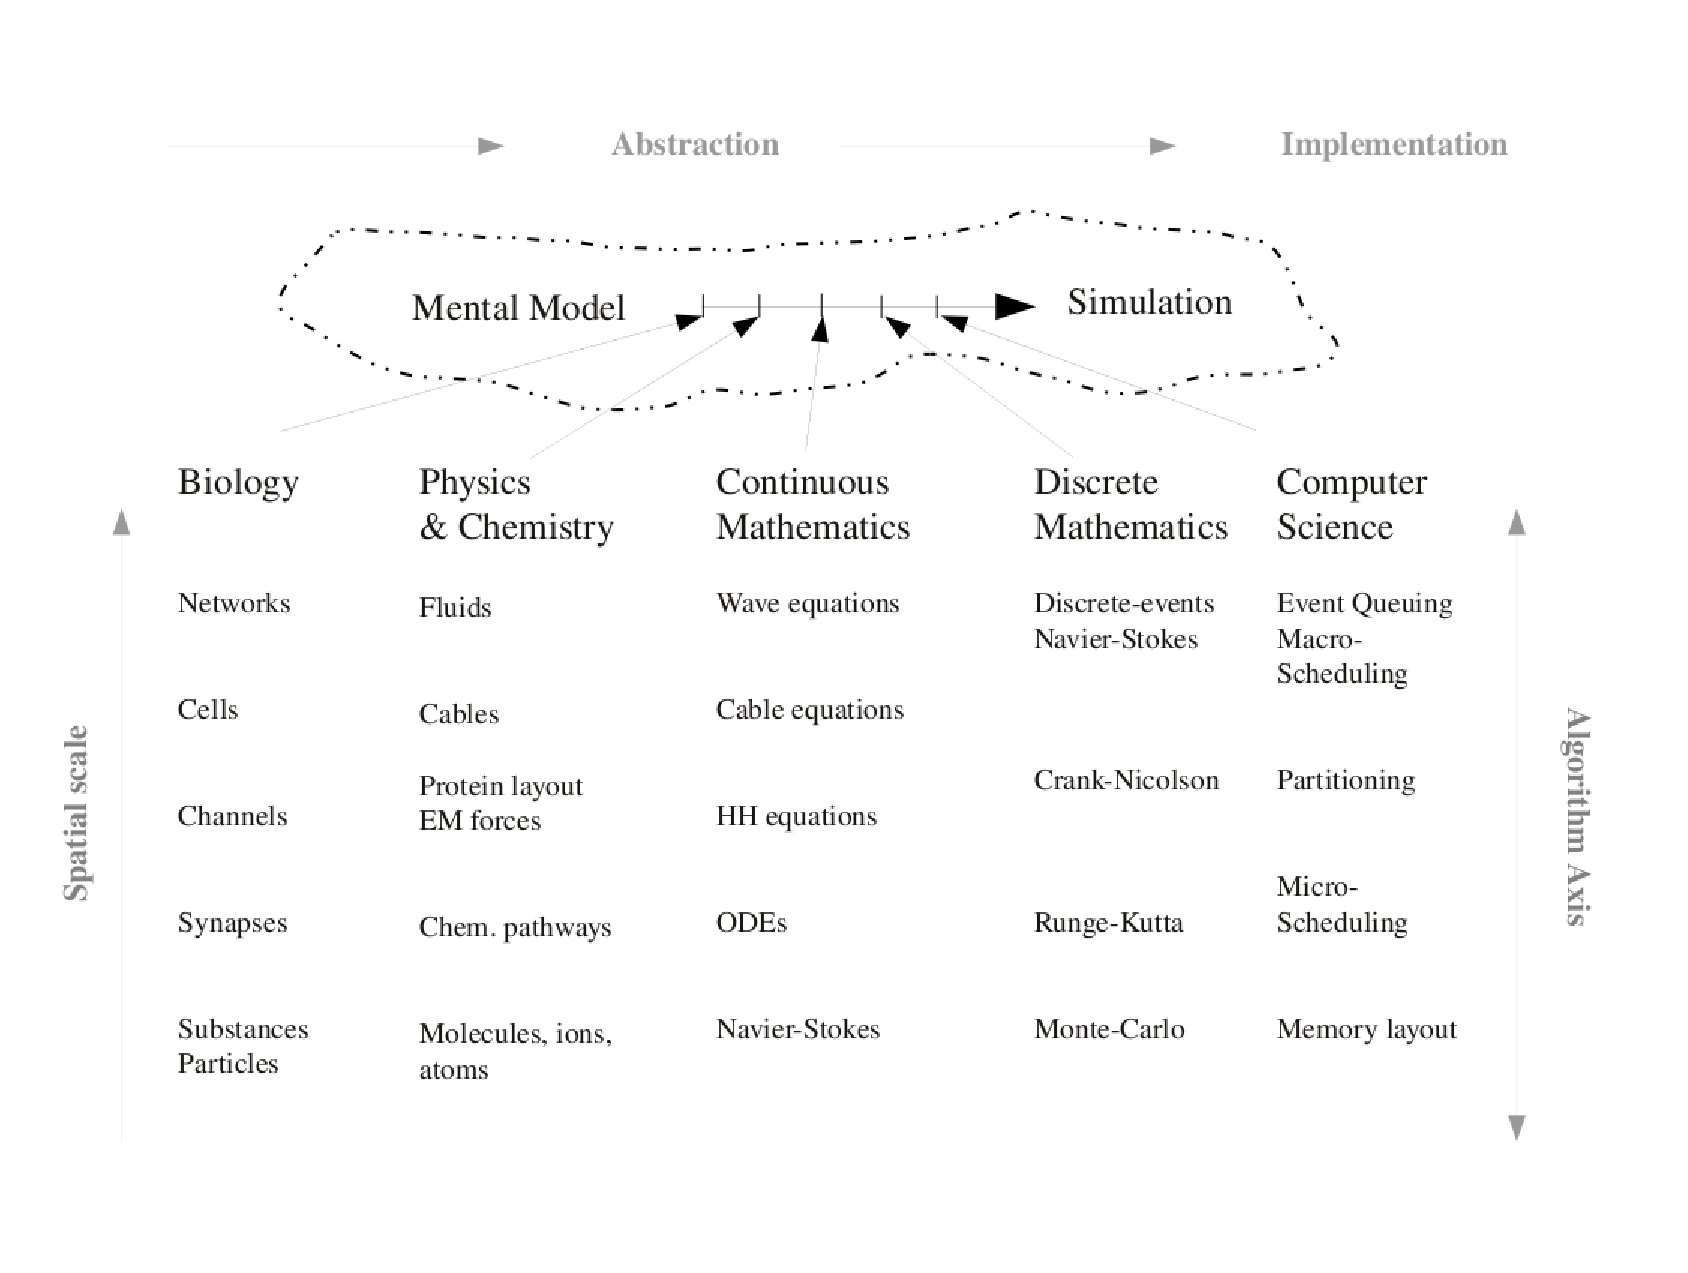
\includegraphics[width=4in]{figures/NS-abstraction-implementation.eps}
  \end{center}
  \caption{ {\bf The Path from Mental Model to Simulation.} }
  \label{fig:mental-model-simulation-path}
\end{figure}



\section*{Methods}

\subsection*{The User Workflow}

The term {\it user workflow}\cite{10.1371/journal.pone.0028956} is
employed to describe the sequence of necessary steps typically
employed by a person in developing a computational model and employing
simulation to generate data for subsequent analysis. In this sense it
is a depiction of a sequence of operations, declared as the work of a
person or a group of persons \cite{Belhajjame:2001fv}.

A comprehensive user workflow can be employed to guide the separation
of the different aspects of a model by organizing user actions into
different categories during model development.  The workflow allows
distinctions to be made between an object under investigation, the
tools used to perform the investigation, and the operations performed
during the investigation. It also distinguishes between the results
obtained from a single investigation and the method used to define
multiple investigations in a series. The user workflow identifies five
steps in total (explained in more detail in Results).

\subsubsection*{The Ideal User Workflow for Simulations in Neurobiology}

As many more data flows can exist than are present in reality, each actual
data flow can be considered in the context of a sequence of user
actions or workflow. We define an ``ideal user workflow'' that provides a canonical form
of a user workflow specific for neural simulators. In this section, we introduce
the set of typical workflows that use CBI simulator architecture
applications by describing the ideal user workflow where a user wants to model a biological system. We then briefly mention a second set of workflows that comprise user extensions of the
functionality of an implementation of the CBI architecture. Both sets of workflows are presented in a technology and implementation free manner.

%In this paper we discuss the first set of workflows by introducing an
%and we superficially touch upon the second
%set of workflows.  All workflows described in the following sections
%are technology and implementation free.
%Examples are given for
%purpose of illustrating the meaning of the text, and neither for
%illustrating the current (state of the existing) implementation, nor
%for a possible implementation in a specific technology.

A five step outline of an ideal user workflow for the development,
implementation, and simulation of a computational model has been
identified from the workflow of users of the GENESIS neural simulation
platform \cite{cornelis02:_tutor}.  Importantly, the workflow
explicitly distinguishes between the static structure of a model of
the biology (Step 1), the dynamic state of its simulation (Step 3),
and the analysis of this dynamic state (Step 4). We also note that
this workflow does not specify any particular order for its
completion. However, for any given case, meaningful simulation output
will only occur with completion of Steps 1--4.

\subsubsection*{Step 1: Construct Model}

The simulator shell and the graphical user interface (GUI) each
provide an interface that interprets user input such that the
simulator `understands' different commands and performs the
appropriate actions. Simple models can be created directly within the
simulator shell by entering a sequence of commands. More complex
models are available to the shell from libraries or databases external
to the simulator. Shell tools can then be used to explore and check
the integrity of a model. Following any necessary or desired changes,
a new version of the model can be saved.

\subsubsection*{Step 2: Design Experiment}

Specific change management tools can be used to make small
modification to a model, e.g. to set model parameter values specific
to a given simulation.  Configuration tools support the definition of
the stimulus or activation parameters for a given simulation run or
experiment and the output variables to be stored for subsequent
analysis by independent software.

\subsubsection*{Step 3: Run Simulation}

Shell tools can be used to check the state of a given simulation or reset the simulation time step and solved variables to their initial values. After a simulation is run, output values are flushed to raw result storage for subsequent data analysis. The model state can be saved at any simulation time step. This allows it to be imported into a subsequent simulator session for further development and exploration.

\subsubsection*{Step 4: Process Output}

The validity and location of simulator output is checked prior to data
analysis. Output can be analyzed either within the simulator or piped
to external applications such as
Matlab. % for subsequent data analysis.

\subsubsection*{Step 5: Iterate}

A modeling project is established by the introduction of iterators
into the user workflow. Iterators close the loop between the output of
results and model construction, they include: Automated construction
of simulations and batch files, static parameter searching, and active
parameter searching using, for example, dynamic clamp technology.


\subsection*{Principal Concerns}

In software engineering, the process of partitioning a program into
logical functions that minimize overlap is referred to as a
{\it separation of concerns}.  We consider that a principled separation of concerns is a prerequisite
for the development of advanced computational modeling techniques in
the neurosciences. User {\it concerns} have a direct influence on the
user's experience of an application.  Technical concerns have a clear
and direct influence on the partitioning of a program into its primary
functional blocks, and are also crucial for problem diagnosis and
guaranteeing the correct behavior of software.  Here, we propose there
are two principal concerns that underly the development of modeling
software: (1) Separation between data and control, and (2) Separation of biology and mathematics through the use of data-layering.

\subsubsection*{Control versus data}
\label{sec:data-vs-control}

All software can be understood in terms of algorithms operating on
input data to produce output data. For experimental research, the
natural distinction between data and algorithms can be compared to the
distinction between the biological system (data to be investigated)
and the stimulation paradigm (tools supporting data investigation).
For computational research, the distinction between data and
algorithms leads to a separation between model (data) and simulation
control (control of data flows).

\subsubsection*{The requirement for data-layering}
\label{sec:data-layering}

%For example, at the biological level,
%a dendritic spine is considered to be a single morphological entity
%but its mathematical equivalent is commonly described by a circuit
%composed of two cable equations: one for the head and one for the
%neck. Similarly, many empirical advances have been made in our
%understanding of the electrophysiological role played by intracellular
%calcium. However, this has frequently been at the expense of
%conflating calcium channel activity with intracellular calcium
%concentrations which, computationally, are at least two distinct
%components of a realistic model. An important consequence is that the
%development of an optimized simulation can be a significant challenge
%for the neuroscientist unfamiliar with mathematical and computational
%theory.

It is the capacity to represent a model in terms of
biological concepts such as neuron, dendrite, soma, channels, and molecules, that
allows a user to clearly relate a model to the original scientific
questions.  One way to achieve this goal is to separate the high-level
biological representation of a model from its low-level mathematical
implementation and provide operators that convert between them.
This insulates the process of model construction
from the computations performed during a simulation. 

The relationships between simulator control and data modules in a federated architecture are symbolized by the horizontal arrows in Figure~\ref{fig:data-control}, whereas the relationship between high level biological concepts and their mathematical implementation are symbolized by the vertical arrows. It is the separation of the principle concerns along the horizontal and vertical axes that allows independent modules to be designed. This process underlies the
construction of a simulator composed of stand-alone
{\it component}s and forms the basic meta-framework
referred to as the CBI architecture.

Importantly, we note that a simulator can be efficiently modularized
when only horizontal or vertical interactions are allowed between the
modules illustrated in Figure~\ref{fig:data-control}. The larger the
number of interactions allowed between diagonally located components,
the more difficult it becomes to functionally separate simulator
components and to maintain and extend the
resulting software application. Diagonal interactions are forbidden in the CBI architecture as they foster the mixing of functionality across different levels that ultimately leads to the creation of monolithic software applications.

%The first implementation of the CBI architecture has been that of  G-3. We use this software platform to present an overview of the CBI federated software architecture through the example of the the new G-3 simulator. In doing this we follow the ideal simulator workflow presented in Methods.

% Figure 2
% \noindent {\bf Place Figure \ref{fig:data-control} about here.}

\begin{figure}[ht]
\begin{center}
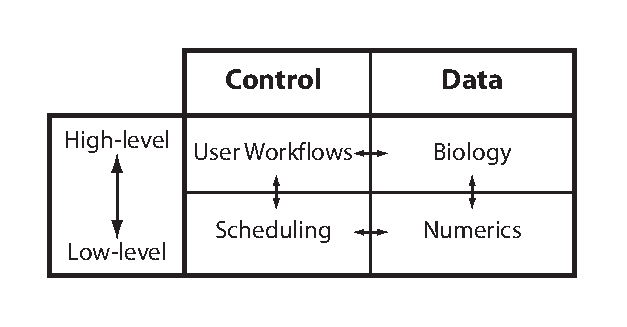
\includegraphics[width=4in]{figures/matrix.eps}
\end{center}
\caption{ {\bf Principle concerns.}  The four fundamental building
  blocks of a simulator are distinguished by separating (i) Data from
  control, and (ii) High level biological concepts from their
  mathematical implementation. In a federated architecture the only
  allowed interactions between modules are those indicated by the
  vertical and horizontal arrows. Diagonal interactions are forbidden
  as they ultimately lead to interactions that result in the existence
  of a monolithic software architecture.
}
\label{fig:data-control}
\end{figure}


\subsection*{Separation of Concerns}

Consideration of the principal concerns of data, control, and data layering were used to expand Figure~\ref{fig:data-control} by the separation of concerns principle. This key principle in software engineering states that a given problem involves different kinds of concerns. To cope with complexity, these concerns should be identified and separated \cite{Dijkstra:1982fu}. The aim is to achieve engineering quality factors such as robustness, adaptability, maintainability, and reusability.  Ultimately, this results in clear model scripts where the biological aspects of a model are separated from the peripheral code that implements a model during a simulation.

% Dijkstra EW (1982) On the role of scientific thought. in Dijkstra, Edsger W.. Selected writings on Computing: A Personal Perspective. New York, NY, USA: Springer-Verlag New York, Inc. pp. 60�66.

In this section we present the outcome of a separation of concerns based on the principal concerns of data- and control-related simulator components introduced above. Initially, the biological and numeric representations and user workflows and scheduling modules are expanded to give the principal functions of the CBI architecture.

Our analysis generated the primary functions of the CBI architecture illustrated in Figure~\ref{fig:cbi-architecture-simple}. The mechanism identified for separation of model construction from the low level computations performed during a simulation was the addition of a mid-level software layer. This intermediate layer provides function and data bindings between scripting applications and database interfaces, respectively, and the low-level back-ends. Note, this figure maintains the relationships between the four principal concerns identified in Figure~\ref{fig:data-control} by separating high level biological representations (Fig.~\ref{fig:cbi-architecture-simple}A) and low level mathematical implementation (Fig.~\ref{fig:cbi-architecture-simple}B), as well as separating control functions from data streams. Note also, the addition of a GUI to connect high level scripting applications with database interfaces.

\subsubsection*{User Workflows and Biological Data}

%Many more possible data flows exist than there are present in reality. So each data flow must be considered in the context of a sequence of user actions or workflow. Initially, the focus is on regular workflows using CBI simulator architecture applications, e. g. where a user wants to model a biological system. We then briefly mention other workflows that support user extensions of the functionality of an implementation of the architecture.
%
The first step in our ideal user workflow involves creating or
importing a model. It maps directly to high-level biological
representations via a simulator shell or GUI.
%Similarly the second
%step in the ideal user workflow allows for the construction and
%management of high-level representations of experimental protocols and
%the physical objects used to implement them.
This interface
straddles the Control/Data divide and replaces the upper horizontal
arrow connecting the {\tt User Workflow} and {\tt Biology} modules in
Figure~\ref{fig:data-control}. It enables the workflow by assisting
either the development of simple cell models from the command line of
a simulator shell via the {\tt Scripting Libraries \& Applications}
module or the importation of model descriptions via the
{\tt Database Interfaces} module (see
Fig.~\ref{fig:cbi-architecture-simple}).
% File formats currently recognized include SWC, the GENESIS P format, the declarative NDF file format, and once finalized, the NeuroML model specification format.

Step 2 of the ideal user workflow typically requires biological
expertise to design an experiment.  This includes the definition of
constants such as the command voltage of a voltage clamp protocol,
delays and duration of a current injection protocol, and model and
simulation inputs and outputs.

%For example given a
%morphology, what are the total surface and volume of the cell, convert
%it to a model, apply current injection into the soma, and record the
%response from a distal dendrite.

\subsubsection*{Numerics and Scheduling}

Step 3 of the ideal user workflow deals with the checking,
resetting, and running of a simulation.  This is accomplished via the
{\tt Function Bindings} module of the CBI architecture (see
Fig.~\ref{fig:cbi-architecture-simple}).
%This module provides a
%mid-level software layer that separates the high level biological
%implementation from the low level numerical implementation of a model
%by providing translators that are capable of making intelligent
%decisions about mapping the given biology to the required numerics.

At a technical level the simulation involves scheduling mathematical
operations on, and communication of, the numerical representations of a
biological model.  This step is indicated by the horizontal arrow
between {\tt Scheduling} and {\tt Numerics} in Figure~\ref{fig:data-control} and
is encompassed by the {\tt Controllers \& Communication} and {\tt Solvers}
modules illustrated in Figure~\ref{fig:cbi-architecture-simple}.

Elaborate user workflows can stop and restart running simulations and
provide new inputs to a model thereby imposing high-level control on
the low-level back-ends via the controller.

\subsection*{Overall Design Objectives}

Several important objectives emerged from the separation of concerns and were used to guide the development
of our federated approach to the design and development of a neuronal
simulation engine. 
% where software components are self contained in the sense that they can be run independently.
They include: (1) Reduced complexity of
software modules when compared to a monolithic system, (2) Simplified
documentation of modules in terms of inputs and outputs, (3) Easy
incorporation or removal of individual modules as required, (4)
Simplified development and testing of modules as stand alone
components, and (5) Clear delineation of scope for new module
development.

\subsection*{Structural Overview of the CBI Architecture}

The CBI architecture is defined as a modular paradigm that places
stand-alone software components into a set of logical relationships.
In this sense it defines a modular framework that provides the
necessary parts of a neural simulator.

The schema identified by the separation of concerns (see
Fig.~\ref{fig:data-control}) is expanded in
Figure~\ref{fig:cbi-architecture-simple} to give the modules that
form the building blocks of the CBI architecture. This figure retains
the four quadrants of simulator functionality identified by our
separation of concerns. It includes the notions of low-level data for
numerics and high-level representations for biology, as well as
separation between data and control
(Fig.~\ref{fig:cbi-architecture-simple} indicated by horizontal and
vertical dashed lines, respectively).
% The CBI architecture draws its
% inspiration from this
% partitioning.

We refer to the CBI architecture
as being `federated' as it extends the modular approach associated
with the development of single applications to the functional
integration of otherwise independent applications. 
Federation aims to provide a unified interface to diverse
applications and mask from the user the differences, idiosyncrasies,
and implementations of the underlying applications and data sources
(see www-128.ibm.com/developerworks/db2/library/techarticle/0203haas/0203haas.html). 
In doing so, federation provides transparency, heterogeneity, a high degree of
function, autonomy for the underlying federated sources,
extensibility, openness, and the possibility of highly optimized
performance. Here, extensibility is defined as a system design principle where an implementation takes into consideration future developments. An extendible system is one that includes mechanisms for expanding or enhancing the system with new capabilities without having to make major changes to the system infrastructure.

Ideally, it makes the underlying applications look like a single
system to the user. Enhanced application interoperability is achieved
through the use of flexible high-level {\it scripting languages} to
support diverse workflows and low-level {\it application programmer
  interfaces} and {\it application binary interfaces} for
performance.
% (see companion paper this issue, Cornelis et al., 2010)\marginpar{ref CBI scripting paper}.

% For completeness, we note that northbound and southbound interfaces
% are indicated in this figure. Northbound interfaces conceptualize
% lower level details, whereas, the southbound interfaces decompose
% the concepts in technical details, which are mostly specific to a
% single component of a software architecture. Northbound interfaces
% normally communicate with southbound interfaces of higher level
% components and vice versa. By convention, north- and southbound
% interfaces are drawn at the top and bottom of an architectural
% overview, respectively.

In summary, the CBI architecture provides a template for software
development that, at its core, contains a simulator.  Additionally,
the modularity and layering of the architecture simplifies connection
to independent applications indirectly related to model construction
and instantiation and the display and analysis of simulation output.
Figure \ref{fig:cbi-architecture-simple} illustrates the various
modules of the CBI
architecture.

% Figure 3
% \noindent{\bf Place Figure \ref{fig:cbi-architecture-simple} about here.}\\

\begin{figure}[ht]
\begin{center}
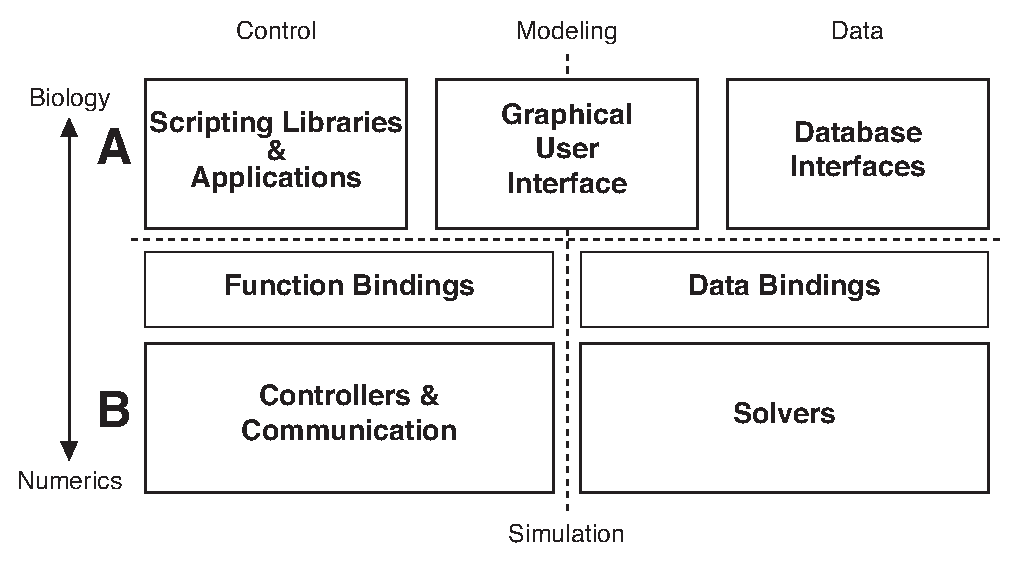
\includegraphics[width=4in]{figures/cbi-architecture-simple.eps}
\end{center}
\caption{ {\bf Overview of a federated software architecture:} Graphical
  illustration of the primary functional modules defined for the CBI
  federated software architecture.  Control modules are given to the left and data modules to the
  right.  A. The top layer contains conceptual data
  and controls representations of the biology of a model. B. The bottom layer contains
  representations that are numeric and thus close to the hardware.  The middle or intermediate layer
  bridges between the biology and the numerics implemented in a CBI compliant simulator. Importantly, as our separation of concerns shows (see Fig. \ref{fig:data-control} and text), Control (Scripting Libraries \& Applications) and Data (Database Interfaces) modules can interact either directly or via the Graphical User Interface.
  }
\label{fig:cbi-architecture-simple}
\end{figure}


\subsubsection*{Behavioural View of the CBI Architecture}

Figure \ref{fig:cbi-architecture-expanded} provides an expanded view
of Figure \ref{fig:cbi-architecture-simple} and illustrates in more
detail the structural relationships between the different modules and
sub-modules that comprise the CBI architecture. We introduced their
functionality above.  The behavior of the CBI architecture is defined
by the functional and dynamic connectivity provided by these
individual modules.  We now describe this behavior within the
context of our ideal user workflow.

% Figure 4
% \noindent{\bf Place Figure \ref{fig:cbi-architecture-expanded} about here.}

\begin{figure}[ht]
  \begin{center}
    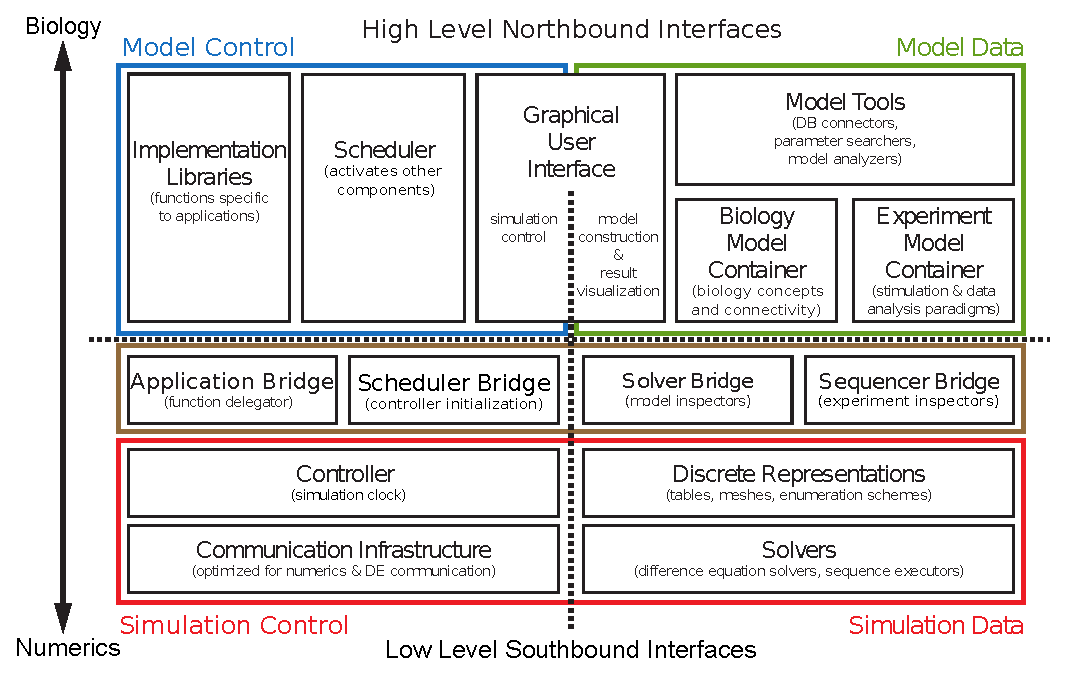
\includegraphics[width=4in]{figures/cbi-architecture-expanded.eps}
  \end{center}
  \caption{ {\bf Detailed view of the Computational Biology Initiative
      federated software architecture.} Illustration of the functional
    modules that is closer to an implementation of the CBI
    architecture. It illustrates the relationships of sub-modules
    within each of the primary functional modules given in Figure
    \ref{fig:cbi-architecture-simple}.  North bound interfaces group
    and conceptualize the details of the modules and interact with
    south bound interfaces of higher level modules.  Steps 1--3 of the
    ideal user workflow induce data flows between the software modules
    of the CBI architecture. This results in data cycling between the
    upper layers (blue and green boxes) and lower layers (red box).
    Ultimately, the two layers team to implement a single simulation.
    By design, any type of model including multi-scale models will
    exhibit this data cycle. See text for explanation and details.
    \vspace{1mm}
    This figure shows a graphical representation of the core structure
    of G-3. In sharp contrast to previous versions of GENESIS and
    other neuronal simulation platforms, the design of G-3 is
    fundamentally modular, separating different functional components
    of the simulator into their own modules. Importantly, G-3
    separates model descriptions from the mathematical representations
    used in actual model simulation.  This simplifies the
    implementation of new solvers and other simulation- time software
    components. The communication infrastructure connects different
    solvers simulating the same model and can 'upscale' or 'downscale'
    numerical data as needed. For additional detail see Cornelis et
    al. 2011a;b.  }
  \label{fig:cbi-architecture-expanded}
\end{figure}


%Steps 1-3 of the ideal user workflow fall within the scope of the
%CBI architecture.
%  Steps 4-5 are outside the CBI architecture and
%cannot induce diagonal connections between the modules inside the
%CBI architecture.

\paragraph{Data-flows in the CBI Architecture}
A (G)UI translates user actions into a family of events that propagate
to other components of a software architecture, impact the internal
states of these components, and direct the data flows between them.
%In the CBI architecture each software component is specialised in
%implementing one particular function and performs the defined
%operations on the data it is passed.
%A functional architecture is an overview of a software system that
%identifies the global functions of the system.  These functions define
%the scope for experts for improvement of the system as a whole.  The
%CBI architecture is structured according to low-level vs. high-level
%functions in the system complemented by the data and control
%functions.  As a consequence, a feature of the CBI architecture is
%that rich data flows occur between software components, but not
%necessarily within them.
In Step 1 (Construct Model) and 2 (Design Experiment) of the ideal
user workflow, users combine models and experimental data that are
stored in files and databases.  In Step 3 (Run Simulation) the
back-ends, such as the numerical {\tt Solvers} and the {\tt
  Communication Infrastructure}, perform the calculations of a
simulation, then save the output back to files and databases.  When
combined, these steps of the ideal user workflow imply a cyclic data
flow from files and databases to the back-ends.  Here we explain how
user actions and data flows relate to one another in the CBI
architecture and define the overall behavior of an implemented
software system.

%Intermediate results may be analyzed or aggregated by
%analysis libraries, e.g. for signal analysis and binning of spikes.
%These libraries are accessible to the CBI architecture from the {\tt
%  Scripting Libraries \& Applications} software component.

%\paragraph{Running a Single Cell Model:}

%When a user wants to learn more about the electrophysiology of an
%existing cell model, it must be instantiated, the stimulation and
%output protocols configured, the simulation run, and the results
%interpreted.

In Step 1 of the ideal user workflow, the GUI is opened and a cell
model is selected from a database listing of available models.
Internally, model selection is translated into an event that instructs
the {\tt Biology Model Container} to load a selected model from a
database and store it in memory using data structures for efficient
storage and retrieval by other modules.  During initial inquiry, a
user may typically be interested in derived model parameters such as
the total surface area of a neuron, with and without spine correction,
while a sophisticated GUI can also present a table of the channels
employed in the model along with their conductance densities and
reversal potentials.  More dedicated queries related to specific brain
areas or neuron types are supported by the {\tt
  Scripting Libraries \& Applications} module.

%A model can be queried in this way when it is stored by
%the {\tt Biology Model Container}.

A typical example of Step 2 of the ideal user workflow is the design
of an experiment that applies current injection pulses to a neuron's
soma and defines simulation output as the somatic membrane potential
and somatic transmembrane currents.  The {\tt
  Experiment Model Container} stores the definition of the current
pulse amplitude and duration, which is translated by a {\tt
  Sequencer Bridge} to a sequence of simulation-time events prior to
the start of a stimulation.  These events are then executed by the
{\tt Command Sequence Executor} during a simulation.

Running the simulation in Step 3 of the ideal user workflow starts
with the {\tt Biology Model Container} examining a stored model to
determine model time constants or other parameters that are relevant
for the accuracy of a numerical simulation.  The {\tt Solvers} then
fill their data structures with parameter values optimized for
simulation, for instance a Crank-Nicolson solver can multiply the
membrane capacitance with the time step during this initialization
phase instead of at every simulation time
step\cite{borg-graham00:_addit_effic_comput_branc_nerve_equat}.  For
this, the memory image of a model must first be expanded into a
representation that includes the mathematical equations and parameters
relevant to the given simulation but, for instance, does not include
the spatial layout of segments as this is not required by the {\tt
  Solvers}.  (Note: `Segment' is a high level term employed to describe different parts of the biological model of a dendritic morphology. The equivalent low level (computational) term is `compartment'. It refers to the numerical representation of a segment.) This behavior is different from that of existing
simulators, e.g. GENESIS 2. Such simulators do not make an explicit
distinction between internal data structures for model representation
and data structures for computation.  Consequently, they often
generate redundant data during the initialization of a simulation.

In network simulations the {\tt Solvers} employ the {\tt
  Connectivity Translator} to initialize its simulation-time
communication data structures and to connect to the {\tt
  Communication Infrastructure}.

When a user instructs the simulator to start a simulation, for
instance by pushing a button in a GUI, the {\tt Controller} generates
a list of instantiated {\tt Solvers}.  It then advances the simulation
clock and requests each {\tt Solver} to update its internal state.
The {\tt Communication Infrastructure} connects the {\tt Solvers} for
efficient communication of the solved variables.  {\tt Solvers} that
were configured for output, save results to a file.  When the
simulation finishes, either by user action or following a preset
simulation period, output buffers are flushed to disk.

The independence of the {\tt Solvers} in the CBI architecture not only
allows for better optimized implementations, but also enables
additional simulator functionality such as serialization of the model
state to a file.  This allows a simulation to be resumed at a later
time and reduces the total simulation time of a complex model if it requires
a calibration phase prior to the application of an experimental
protocol.

%During Step 4 the dynamic state of the model is available from the files and databases for further analysis.

% Steps 4 and 5 are complementary to Steps 1-3 of the ideal user workflow.

%The data cycle between databases and files, and the solvers in Steps
%1-3 of the ideal user workflow results in all simulation simulation output
%is available through these databases and files.  Once these steps
%have been completed, the back-ends of the CBI architecture are not
%available anymore.  The simulation result data can then be combined
%with the model parameters and structure available in the {\tt
%  Biology Model Container} through {\tt
%  Scripting Libraries \& Applications} to implement Step 4 and 5 of
%our ideal user workflow.

As a result of Steps 1--3 of the ideal user workflow, data flows both
through and between software components that conform to a CBI
architecture: the data cycles between databases and files, and
back-end {\tt Solver}s.  Here we have described this cycle for a single
neuron model and, as we briefly noted, it also occurs for network
models.  By design any type of model including multi-scale models
will exhibit this data cycle.

In Steps 4 and 5, the availability of any model data from the {\tt
  Model Container} and the functionality of {\tt
  Scripting Libraries \& Applications} can connect the CBI
architecture with external tools while maintaining the integrity of
the separation of concerns.
%The laterality of the software component connectivity activated during Step 4 is not an issue.
{\tt Scripting Libraries \& Applications} connect to external tools
such as Matlab to implement output analysis.
%  Integration, at Step
%4 of the ideal user workflow, with software platforms such as RTXI
%make direct interaction with experiment possible.
They also allow simulation output data to be combined with the model
parameters and structure available in the {\tt
  Biology Model Container} to implement Step 5 of our ideal user
workflow, for instance to provide automated script generators for the
generation of batch simulations.  Importantly, at this stage of the
workflow, the back-ends of the CBI architecture (indicated below the dotted
horizontal line in Figures~\ref{fig:cbi-architecture-simple}
and~\ref{fig:cbi-architecture-expanded}) are unavailable.  Once Step 3
is completed, all the data of the dynamic state of the model are
available through databases and files.  Consequently, there is no
requirement to query the software components that deal with
numerical data. This ultimately prevents the implementation of
diagonal interactions in the software and the creation of a monolithic
simulator.

% are technically unrelated to a simulation run and may
%fall outside the scope of the CBI architecture.  On the other hand
%{\tt Scripting Libraries \& Applications} may connect to external
%tools such as Matlab to implement output analysis and include script
%generators for automation of batch simulations and platforms such as
%RTXI for a direct connection with experiments.

%For convenience one could implement a short-cut diagonal into the CBI
%architecture for implementation of aspects of Steps 4 and 5, and for that matter other Steps, but this ultimately would limit the functional scope of the resulting simulator.

%All model data is available through the model container and the output (files or databases).  

%Modules plugged in during Step 4 have access to all data via the model container.

\subsection*{GENESIS 3.0}


The redesigned and modernized core structure of GENESIS produces
GENESIS version 3.0 or G-3.  The new structure of G-3 provides a new
and unique capacity for federated and modular software development in
support of multi-scale modeling.  Furthermore, G-3s structure also
supports the direct real time interaction, or embedding of models at
different levels of scale.  As described in more detail below, this is
accomplished through specific software modules that create
intermediary representation of variables present at multiple scales as
described in more detail in subsequent sections.

Several explicit features of G-3 allow the rapid incorporation of new
software components.  As illustrated below these include: 1) the
modular separation of the development of the core of new solvers from
that of other software components, allowing full focus on the
mathematical aspects of the solver and their implementation, and
better optimization; 2) the G-3 Developer package facilitates
integration of the Chemesis-3 solver into the build system of G-3
enabling immediate regression tests; 3) easy extension of the
configuration of the model-container to establish new declarative
model tokens and parameters recognized by the Chemesis-3 solvers; 4)
easy construction of an interface between the model-container
application programmers interface (API) and the core of the Chemesis-3
solver and finally 5) the specific development of a communication
software component that interfaces the new solver with the existing
linear cable solver.

Because each of these sub-cellular modeling components are an
integrated part of a single model-container (see Cornelis 2011a), the
existing and new G-3 solvers can be integrated to simulate different
aspects of the same model.  This 'scale-linking' functionality of G-3
instantiates dedicated run-time software components that contain
intermediary representations of solved variables that can pass both
'upscale' and 'downscale' values to solvers at different levels of
scale.  Technically, in the case of Chemesis-3 and the linear cable
solver, for example, these modules calculate weighted space-time
averages.


\subsection*{Extending GENESIS-3}

The G-3 documentation systems describes the procedures used for G-3
extension.  Extending G-3 can involve the implementation of a new
solver, or, when the required functionality is tangential to an
existing solver, it can require source code additions to an
pre-existing software component.  Here we describe the integration of
a new solver, ie. the steps followed for the implementation of
Chemesis-3.

  1. The developer package integrates the different software
  components of G-3.  The definition of a new component "chemesis3" in
  the developer package allows for its smooth integration with other
  G-3 software components such as the model-container.

  2. The implementation of the core of a new solver is independent of
  the development of other software components.  This allows full
  focus on the mathematic aspects of the solver and their
  implementation.

  3. Optionally, the model-container can be extended with new tokens
  that are specific to the new solver.  Configuration of the
  model-container defines the new tokens and their parameters.

  4. An interface must be written between the model-container and
  the core of the solver.  The model-container defines an API that
  makes abstraction of the biological structure the model.


\subsection*{Heccer: A Numerical Solver}

% example: direct link to external documentation
%
%Uses the
%\href{http://www.neuron.yale.edu/ftp/neuron/papers/effic84.pdf}{Hines
%  enumeration algorithm} for efficient solution of the cable matrix.

% example: link to external documentation using a redirect
%
%Uses the
%\href{../effic84/descriptor.yml->redirect}{Hines
%  enumeration algorithm} for efficient solution of the cable matrix.

The optimization of a neuronal solver ultimately focuses on accuracy and performance. Transforming complex biological parameters into precomputed tables and optimizing for a high CPU cache hit ratio are the most important features for a good solver, and gives the solver a performance boost of about a factor four to six.

{\bf Heccer} is a fast compartmental solver, that is based on {\it hsolve} of the GENESIS simulator. To find out more about the numerical principles implemented in {\bf Heccer} see \href{http://www.genesis-sim.org/GENESIS/gum-tutorials/cornelis/doc/html/node3.html}{a small tutorial on numerical theory}. The efficiency of {\bf Heccer} is explained in \href{http://www.genesis-sim.org/GENESIS/gum-tutorials/cornelis/doc/html/node53.html}{Byte Code Compilation}.

{\bf Heccer} can be instantiated from C, or from Perl (or other scripting languages). It is also possible to link {\bf Heccer} directly to Matlab. {\bf Heccer} comes with \href{http://www.swig.org/}{\bf Swig} interface definitions, such that linking {\bf Heccer} to any other technologies should be easy.

Adding new channel types to {\bf Heccer} can be done using callouts.
The callout mechanism allows for general user extensions that
contribute a current or conductance at a particular time in a
simulation. {\bf Heccer} automatically integrates this contribution
into the membrane potential.  Check the tests of the callouts for more
information (tests/code/callout1.c and tests/code/calloutInjector.c).

The source code of {\bf Heccer} contains inline developer documentation. As yet, there is no stable API but the Swig interfaces for {\bf Heccer} are not expected to change much. If you are interested in this, look at \href{http://neurospaces.sourceforge.net/neurospaces_project/heccer/tests/html/glue/swig/perl/fork4p1.source.html#line51}{a simple example} for driving {\bf Heccer} from Perl, and \href{http://neurospaces.sourceforge.net/neurospaces_project/heccer/tests/html/glue/swig/perl/pool1-feedback1.source.html#line51}{another example} with active channels and a calcium pool. {\bf Heccer} is currently capable of simulating Purkinje cells (see the \href{../purkinje-cell-model/purkinje-cell-model.tex}{\bf Purkinje\,Cell\,Model}), and, at first evaluation, runs slightly faster than {\it hsolve} (It is difficult to assess why exactly: while the {\it hsolve} implementation is much more optimized than {\bf Heccer's}, the {\bf Heccer} design is slightly better optimized than {\it hsolve}'s.).

\subsubsection*{Heccer Features}

\begin{itemize}

\item Can be driven from C, Perl, SSP, and fetches the model
  parameters from the
  \href{../model-container/model-container.tex}{\bf Model\,Container}.
  The test specification in the Heccer package have examples of
  C-level tests (see the tests/code/ directory) and Perl-level tests
  (check the tests/glue/swig/perl/ directory).  The SSP package
  defines many tests that integrate Heccer and the model-container.
\item Computes the behaviour of single neurons.
\item Integrates Hodgkin-Huxley-like channels.
\item Integrates exponentially decaying calcium concentrations and Nernst potentials. Interfaces will be provided for more elaborate calcium models.
\item Can operate in a ``passive-only'' mode, i.e. all channels in a model are ignored with exception of the synaptic channels.
\item Tables to speed up computations, are dynamically generated and optimized.
\item All parts of a model with the same kinetics automatically share tables.
\item Computes the contribution of one channel type to the overall dendritic current, e.g. the contribution of all calcium channels or the contribution of all persistent calcium channels.
\item Can serialize the current neuron state to an external stream for later resuming the simulation (or for multiple use).
\item Generalizing the previous point, can be initialized from external sources.
\item Can be used with or without the {\bf Model\,Container}. To use {\bf Heccer} without the {\bf Model\,Container}, configure the module with the command line ``{\tt ./configure --without-neurospaces}''. To use {\bf Heccer} with the {\bf Model\,Container}, the {\bf Model\,Container} must be installed before {\bf Heccer} is compiled. 
\end{itemize}
{\bf Heccer} has been validated with a Purkinje cell model and produces an exact match with {\it hsolve} (see the purkinje cell model and the Purkinje cell tutorial in the GENESIS simulator distribution). {\bf Heccer} is constantly undergoing regression tests. Link to  \href{http://neurospaces.sourceforge.net/neurospaces_project/heccer/tests/html/index.html}{\bf Regression\,Test\,Output}. These tests give an idea of the functionality of {\bf Heccer} as a compartmental solver.

Besides being open source, {\bf Heccer} is also hypersource and \href{http://repo-genesis3.cbi.utsa.edu/crossref/heccer/heccer/index.html}{\bf Heccer\,Source\,Code} is browsable.
% An example test file with points of entry into {\bf Heccer}, can be found \href{}{here}.

\subsubsection*{Extending Heccer}
\begin{itemize}
   \item Adding new channel types to {\bf Heccer} can be done using
     callouts.  The callout mechanism allows for general user
     extensions that contribute a current or conductance at a
     particular time in a simulation. {\bf Heccer} automatically
     integrates this contribution into the membrane potential.  Check
     the tests of the callouts for more information
     (tests/code/callout1.c and tests/code/calloutInjector.c).
%   \item \href{../genesis-add-object-solver/genesis-add-object-solver.tex}{\bf Create and Add New Solver Object:} Shows by example how to add a new simulation object to {\bf Heccer} and integrate the modified component with GENESIS.
%   \item \href{../genesis-add-swigbinding-heccer/genesis-add-swigbinding-heccer.tex}{Add a SWIG binding to {\bf HECCER:}} Shows by example how to implement the necessary bindings to make a \href{../simulation-objects/simulation-objects.tex}{\bf Simulation\,Object} callable from Perl using SWIG.
\end{itemize}


\subsection*{Chemesis-3}

NOTE: this section is written as structured text instead of latex.

*Chemesis* is a G-2 'add-on' library of objects for modeling biochemical
reactions, models of second messengers, and calcium dynamics, created by K.
T. (Avrama) Blackwell (2000).  As a test case for user-extensibility of G-3
we began implementing the Chemesis library as a G-3 software component.
Our goal was to determine how difficult and time-consuming it would be to
implement a new G-3 software component *chemesis3* based on a G-2
implementation of a set of new objects.  The original implementation relied
on the generic G-2 numerical solver.  Only limited time was available for
the implementation of the specialized chemesis-3 solver.  A time line
reconstructed from the email conversations and from the version control
system shows the course of development:

- exploratory email conversations May 30th and following two weeks.

- initial preparations and start of implementation on June 13th.

- core implementation on Sunday June 26th, including a fully working
  cal1 regression test case.  This was a day of crazy coding as in the
  old days, total of 18 revisions with many enhancements.

- implementation of cal2 test case on June 29th and July 10th.

- initial scripting bindings were added starting at July 10th for perl
  and July 13 for Python.

- first successful integration with the SSP scheduler on July 12th.

- model-container bindings started on July 13 and finished on July
  17th.  Removed model-related functions such as compartment volume
  computation that are already available in the model-container (and now
  shared with other solvers).

- G-shell integration on July 17th and July 18th.

The objects currently implemented in the G-3 *chemesis3* component are:

*rxnpool*: a concentration pool that interacts with reactions and
diffuses to other pools. (Maps to NDF token POOL.)

*conservepool*: mass conservation based pool, computes the difference
between the total of all molecules (a model parameter, rest state),
and diffused molecules, divided by compartment volume.
(Maps to NDF token POOL, with a different parameterization.)

reaction: standard forward / backward chemical reactions between pools
of molecules. (Maps to NDF token REACTION.)

*diffusion*: Computes flux in molecules between two pools.
(Maps to NDF *segment parameter* diffusion\_constant.  The appearance of
this parameter in an NDF file requires running the model using a
chemesis3 solver.)


\section*{Results}

\subsection*{Simple Python Scripting}

- CBI-scripting, python scripting.

\subsection*{Scripting Chemesis}

- Chemesis CNS report.

Our goal was to implement and run two of the G-2 Chemesis tutorial examples.

The example script *cal1.g* creates a single compartment with interaction
between calcium and a buffer.  A second example *cal2.g* creates a two
compartment model with a dendrite and soma. One additional diffusion object
is required to allow for diffusion between compartments.

The two listings below show the G-2 SLI language script *cal1.g* and the G-3
NDF representation *cal1.ndf*, found with *cal2.ndf* in
'/usr/local/neurospaces/models/library/chemesis'.


**cal1.ndf**::

\begin{verbatim}
#!neurospacesparse
// -*- NEUROSPACES -*-
NEUROSPACES NDF
// VERSION 0.1
PUBLIC_MODELS
  KINETICS cal1
    PARAMETERS
      PARAMETER ( DIA = 24e-4 ),
      PARAMETER ( LENGTH = 24e-4 ),
    END PARAMETERS
    POOL somaCa
      BINDABLES
        OUTPUT concen
      END BINDABLES
      PARAMETERS
        PARAMETER ( concen_init = 0.001 ),
        PARAMETER ( DIA =  ..->DIA ),
        PARAMETER ( LENGTH =  ..->LENGTH ),
        PARAMETER ( "UNITS" = 1e-3 ),
      END PARAMETERS
    END POOL
    POOL somaCabuf
      BINDABLES
        OUTPUT concen
      END BINDABLES
      PARAMETERS
        PARAMETER ( concen_init = 0.003 ),
        PARAMETER ( DIA =  ..->DIA ),
        PARAMETER ( LENGTH =  ..->LENGTH ),
        PARAMETER ( "UNITS" = 1e-3 ),
      END PARAMETERS
    END POOL
    POOL somabuf
      BINDABLES
        OUTPUT concen
      END BINDABLES
      BINDINGS
        INPUT ../somaCabuf->concen,
      END BINDINGS
      PARAMETERS
        PARAMETER ( concen_init = 0.153 ),
        PARAMETER ( concen_total = 0.153 ),
        PARAMETER ( DIA =  ..->DIA ),
        PARAMETER ( LENGTH =  ..->LENGTH ),
      END PARAMETERS
    END POOL
    REACTION somacabufrxn
      BINDABLES
        INPUT concen, OUTPUT concen
      END BINDABLES
      BINDINGS
                    INPUT ("substrate") ../somaCa->concen,
        INPUT ("substrate") ../somabuf->concen,
        INPUT ("product") ../somaCabuf->concen,
      END BINDINGS
      PARAMETERS
        PARAMETER ( FORWARD_RATE = 1e2 ),
        PARAMETER ( BACKWARD_RATE = 0.5 ),
      END PARAMETERS
    END REACTION
  END KINETICS
END PUBLIC_MODELS
\end{verbatim}


The commands below illustrate how the G-3 Studio (model explorer) is used
to load  *cal1.ndf* into the Model Container and explore the model::

\begin{verbatim}
  \$ genesis-g3
  Welcome to the GENESIS 3 shell
  genesis > ndf_load /usr/local/neurospaces/models/library/chemesis/cal1.ndf
  genesis > explore
\end{verbatim}

[chemesis-cal1.png - sent by Hugo]
[chemesis-cals.png - sent by Hugo]

[if possible -  G-shell commands to run cal1.ndf and output to a file]



\subsection*{Multiscale Scripting}

The details of the procedure followed can be seen in the online
documentation "G-3 Extension" (genesis-extend-functionality) and
"chemesis-3-log".


Different numerical solution methods are required to solve the different
types of mathematical equations associated with different scales of
modeling.  The cable equation and ion currents are numerically solved with
implicit Crank-Nicolson integration.  In G-3 this method of solution is
implemented in a dedicated compartmental solver called Heccer.  In the G-3
shell the user has to create a mapping from the name of the neuron model to
the solver.  In the past, this was not necessary, as Heccer was the only
solver.  Under planned extensions to the G-shell syntax, the correct syntax
for a loaded single neuron model with name "/traub94" would be::

  genesis > solverset "/traub94 => heccer"

Biochemical pathways in neuronal modeling are complex networks of
interacting ion concentration pools.  The G-3 implementation for
simulation of biochemical pathways is called Chemesis-3 and has a
dedicated optimized implementation to represent networks parameterized
with biochemical pathways.  To simulate a complex network model of
biochemical pathways, in this example called "/cal1", a user would
typically type from the G-3 shell::

  genesis > solverset "/cal1 => chemesis3"

In case the network of biochemical pathways is defined inside the
single neuron model, a user would have to type two commands with
wildcards that associate the correct solver with each component of the
model, for example::

  genesis > solverset "/**/cal1 => chemesis3"
  genesis > solverset "/traub94/**[!cal1] => heccer"

In later version of G-3 these rules will be built in but still allow
the user to select a different method of solution for different
components of his or her model.


* VERY brief list of steps or description of steps to convert chemesis

  1. Creating a new component "chemesis3"

  2. Creating a new object within an existing "chemesis3".
     "model-container", or "experiment" module

  [Hugo, I will need some help here.  This can be very short, although
  we had originally meant it to be a major part.  Perhaps the first item
  can be glossed over for this audience.]

\subsection*{Multi-scale modeling support in G-3}

Supported types by the model-container:

- Grid3D / Populations / Networks

- VolumeConnect / Individual Connections

- Single Cells / Morphology

- HH - Channels / Synaptic (NMDA / AMPA) Channels

- Reaction -- Diffusion


Available solvers, starting at the highest scale:

- DES: discrete event queuing and distribution

- Heccer: single neuron solver.

- Chemesis-3: simple reaction-diffusion systems,

- Experiment: current injections, time-tables and output.


\section*{Discusion}

- Summary.

- Parts of the multiscale grant.

The definition of the multi-scale modeling as used in this paper
allows to define a taxonomy of models in computational neurobiology
based on both the biological scale of a model and the level of detail
it aims to represent (figure~\ref{fig:multi-scale-taxonomy}).

\begin{figure}[ht]
  \begin{center}
    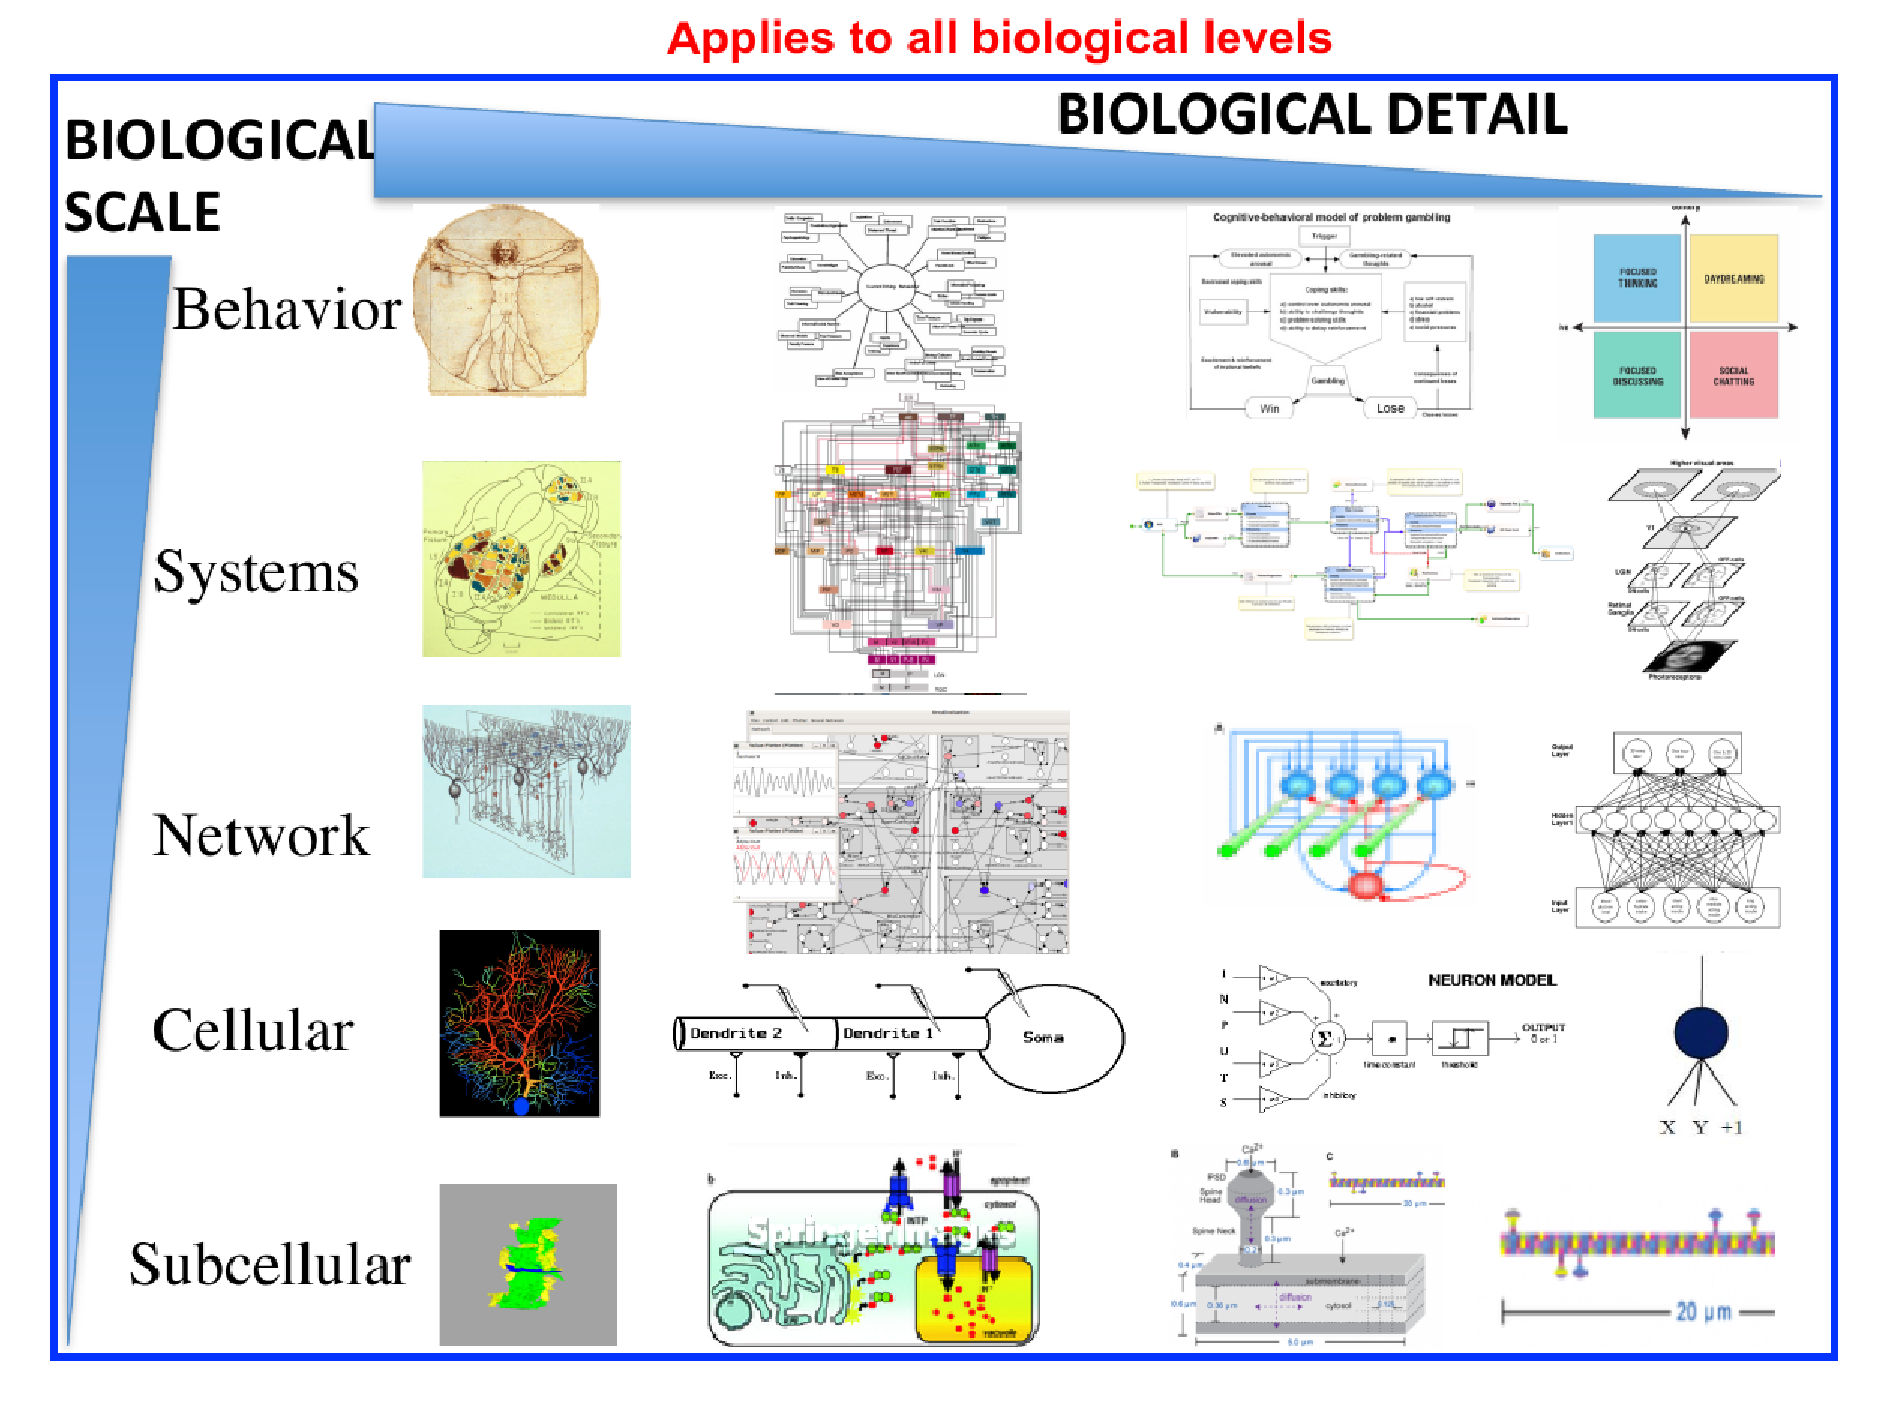
\includegraphics[width=4in]{figures/multi-scale-taxonomy.eps}
  \end{center}
  \caption{ {\bf Taxonomy of Multi-scale Models.} }
  \label{fig:multi-scale-taxonomy}
\end{figure}


Incorporate two types of 3-D Monte Carlo-based techniques for modeling
reaction/diffusion kinetics. Specifically, Dr. Avrama Blackwell will
work with the G-3 development team to implement NeuroRD (Oliveira et
al., 2010), a computationally efficient approximate Monte Carlo
approach to modeling reaction-diffusion systems.

In addition, the G-3 development team will work with Dr. Yoshi Kubota
to incorporate 'CDS' (Cellular Dynamics Simulator:
http://nba.uth.tmc.edu/cds/) a precise particle-based Monte Carlo
simulator specifically supporting the modeling of Ca2+ binding and
diffusion dynamics within biochemical networks (Byrne et al. 2010;
Kubota and Waxham 2011). CDS is based on the event-driven first
passage time algorithm (Byrne et al. 2010) and is designed to serve as
a flexible platform for multi-scale hybrid algorithms.  For this
reason, the CDS algorithm can be directly combined with any
deterministic ODE/PDE (Reaction-Diffusion Equation) solvers (e.g.,
V-Cell used in Hernjak et al. 2005) including those already included
in G-3.  High-resolution cellular morphology including that of
dendritic spines can be directly transported to CDS allowing
electro-diffusion to be simulated by both deterministic (as in
Lopreore et al. 2008) as well as particle-based 3-D stochastic
methods.

This will allow us to compare different simulation algorithms for Ca2+
binding diffusion, voltage clamp, and biochemical network within the
same platform and will help derive and validate simplified macroscopic
(biochemical) synaptic rules relevant to the objectives of Specific
Aim 2.

From a technical point of view, the incorporation of simulations
modules that specifically involve spatial dimensions is, in principle,
much more difficult than the integration of biochemical kinetic
models. In fact the accurate representation of space and time for
multi-scale simulations is an open research area.  However, the
explicit provision of software modules for the intermediary
representation of solved variables allows to compare and evaluate
different methods of scale-linking, for instance by comparing
different resolutions of a fixed grid with adaptive grid intermediary
representations (Bernabeul et al., 2009). In effect, this will allow
us to use multi-scale G-3 models as a framework to compare different
technical strategies.

G-3 supports the construction of very large scale network and system
models based on more abstracted neuronal components.  In support of
this function, the G-3 model-container applies specific algorithms to
instantiate systems level connectivity models and convert them to
mathematical representations, relieving the mathematical solvers from
the pressure typical for rich heterogeneous model structures.  At the
same time, the intermediate simulation system modules already
described as the mechanism used to link Chemesis-3 and the linear
cable solver, will also be used to share values and functions between
larger scale network simulations and lower scale models.  The long
term (Nelson et al., 1989; De Schutter and Bower, 1992) and intrinsic
support for use of parallel computing resources within the GENESIS
system will also be critical to the ability to run large scale models
(Cornelis 2011a; b) with the large scale simulations being carried out
on Linux clusters of 100-500 CPU cores.


\subsection*{text sources}

- email jim single model -container

- multiscale grant

- dave's chapter

- chemesis cns report

- two papers


\subsection*{additional references}

Blackwell, K. T. (2000) Evidence for a Distinct Light-Induced
Calcium-Dependent Potassium Current in Hermissenda Crassicornis,
J. Computational Neuroscience, 9: 149-170.

DeSchutter, E., and Bower, J.M. (1994)  An Active Membrane Model of the
Cerebellar Purkinje Cell: I simulation of current clamps in slice   J.
Neurophysiol.  71:375-400.

Kotaleski, J. H., Plenz, D. and Blackwell, K. T. (2006) Using potassium
currents to solve signal-to-noise problems in inhibitory feedforward
networks of the striatum. J. Neurophysiol.  95: 331-341.

- dave's chapter

- visual interface to neuron (see Jim's review invitation)

- numerical solvers, see Andrew Davison's email.


%\begin{figure}[h]
%  \centering
%   
\includegraphics[scale=0.5]{figures/dummyfig.eps}
%\caption{{\bf A Dummy Figure:} Example of \LaTeX\,\,\,code to incorporate a figure into documentation.}
%  \label{fig:df-2}
%\end{figure}

\bibliographystyle{plain}
\bibliography{../tex/bib/g3-refs.bib}

\end{document}
